\documentclass[UTF8,12pt]{ctexart}
 
\usepackage{listings}
\usepackage{xcolor} 
\usepackage{hyperref}
\usepackage{graphicx}
\usepackage{booktabs} %绘制表格
\usepackage{caption} %标题居中
\usepackage{geometry}
\usepackage{array}
\usepackage{amsmath}
\usepackage{subfigure} 
\usepackage{longtable}
\usepackage{abstract}
\pagestyle{plain} %页眉消失
 
\geometry{a4paper,left=2.5cm,right=2.5cm,top=2.5cm,bottom=2.5cm}
\lstset{
		numbers=left, %设置行号位置
		numberstyle=\tiny, %设置行号大小
		keywordstyle=\color{blue}, %设置关键字颜色
		commentstyle=\color[cmyk]{1,0,1,0}, %设置注释颜色
		escapeinside=``, %逃逸字符(1左面的键),用于显示中文
		breaklines, %自动折行
		extendedchars=false, %解决代码跨页时,章节标题,页眉等汉字不显示的问题
		xleftmargin=1em,xrightmargin=1em, aboveskip=1em, %设置边距
		tabsize=4, %设置tab空格数
		showspaces=false %不显示空格
	}
 

% 用来设置附录中代码的样式

\lstset{
    basicstyle          =   \sffamily,          % 基本代码风格
    keywordstyle        =   \bfseries,          % 关键字风格
    commentstyle        =   \rmfamily\itshape,  % 注释的风格,斜体
    stringstyle         =   \ttfamily,  % 字符串风格
    flexiblecolumns,                % 别问为什么,加上这个
    numbers             =   left,   % 行号的位置在左边
    showspaces          =   false,  % 是否显示空格,显示了有点乱,所以不现实了
    numberstyle         =   \zihao{-5}\ttfamily,    % 行号的样式,小五号,tt等宽字体
    showstringspaces    =   false,
    captionpos          =   t,      % 这段代码的名字所呈现的位置,t指的是top上面
    frame               =   lrtb,   % 显示边框
}

\lstdefinestyle{MATLAB}{
    language        =  MATLAB, % 语言选MATLAB
    basicstyle      =   \zihao{-5}\ttfamily,
    numberstyle     =   \zihao{-5}\ttfamily,
    keywordstyle    =   \color{blue},
    keywordstyle    =   [2] \color{teal},
    stringstyle     =   \color{magenta},
    commentstyle    =   \color{red}\ttfamily,
    breaklines      =   true,   % 自动换行,建议不要写太长的行
    columns         =   fixed,  % 如果不加这一句,字间距就不固定,很丑,必须加
    basewidth       =   0.5em,
}

\lstdefinestyle{python}{
    language        = python, % 语言选python
    basicstyle      =   \zihao{-5}\ttfamily,
    numberstyle     =   \zihao{-5}\ttfamily,
    keywordstyle    =   \color{blue},
    keywordstyle    =   [2] \color{teal},
    stringstyle     =   \color{magenta},
    commentstyle    =   \color{red}\ttfamily,
    breaklines      =   true,   % 自动换行,建议不要写太长的行
    columns         =   fixed,  % 如果不加这一句,字间距就不固定,很丑,必须加
    basewidth       =   0.5em,
}


\begin{document}
\begin{table}[htbp]
\zihao{4}
	\centering
	\caption*{} 
	% l 左 c 居中 r 对齐
	% | 竖线 \hline横线 || 双竖线 \hline \hline 双横线
	\begin{tabular}{| l |c|c|c|}
		\hline
		参赛队名称 &\multicolumn{3}{|c|}{天问} \\
		\hline
		参赛队单位 & \multicolumn{3}{|c|}{数学与统计学院} \\
		\hline
		参赛队员 &\multicolumn{3}{|c|} {马程远}\\
		\hline
		联系人 & 姓名:马程远 & 邮箱:1552650018@qq.com & 电话:18770500186\\
		\hline
	\end{tabular}
\end{table}
\vspace{30pt}

\begin{center}
	

\zihao{-0}\textbf{中南大学第二届先进飞行器虚拟仿真大赛}

\begin{figure}[htb]
	\centering
	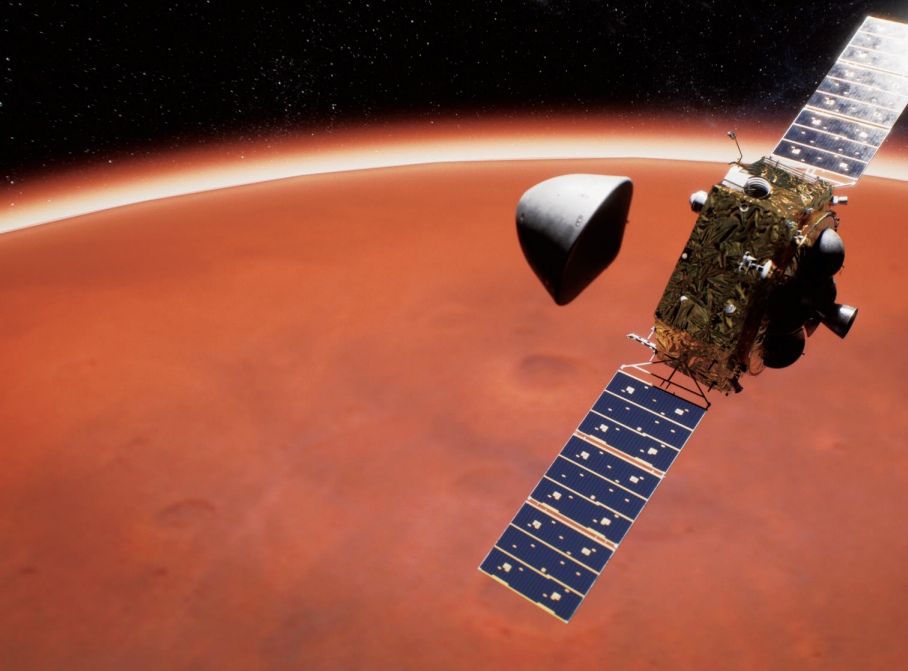
\includegraphics[width=0.8\linewidth]{天问.png}
	\caption*{}
	\label{fig:pathdemo}	
\end{figure}

\vspace{50pt}
\zihao{-3}{日期:2021年10月28日}


\newpage
\tableofcontents
\end{center}
\newpage
\section{设计理念的概述}
	自古以来人类不断探索宇宙的奥妙,为解开宇宙和生命起源付出了一代代的努力。
随着航天技术的不断进步,人类从探月工程迈向火星计划,不远的将来人类一定有能力
走出太阳系,在更加浩瀚的宇宙中自由穿行。


深空探测具有非常重要的科学研究价值和现实意义,可以为地球资源枯竭提供有效
解决途径,为揭开宇宙和生命起源提供科学依据,同时对发现新物质和科学研究具有不
可替代的作用。火星探测是近年来深空探测领域的热点,而无论是当前的着陆探测火星阶段还是未来的采样返回和载人探测火星阶段,
都需要火星探测器能够安全地着陆在预先选择的具有较高科学价值的预选点处,
这就迫切地需要未来火星探测器的着陆系统具有较高的着陆精度。

由此,本作品以天问一号探测器着陆火星为背景,
对火星着陆飞行器的着陆轨迹设计进行了分析研究。

首先建立了常用的坐标系和运动变量及转换关系,介绍了火星探
测着陆器和降落伞的几何构型,在火星大气模型及相应的不确定性模型的基础
上,对着陆巡视器飞行的力学环境进行了建模,包括火星引力、着陆器和降落伞
在不同阶段所受到的不同的气动力模型、控制力模型等。

本作品对飞行器的轨迹优化考虑状态约束与路径约束,采用火星重力场模
型推算给出大气层进入位置为时间指标的最优进入轨迹,并分析了进入角约束
对进入轨迹的影响;飞行着陆器进入火星大气后制导受火星环境影响较大,本作品考
虑火星大气不确定性,建立火星大气模型,通过火星卫星气动下降以及降落伞模
拟仿真分析了制导律的稳定性和精度,对环境不确定性展开了分析,评估了开伞
过程中峰值力和力矩对伞舱组合体动力学性能的影响。
接着通过火星 EDL 过程的环境模型、动力学模型及制导控制方法,进行了
火星 EDL 全过程一体化仿真,可以对进入、下降与着陆各阶段进行仿真验证。

对于着陆器飞行器轨迹的设计,本作品首先对飞行器分离轨道的初始点和着陆点进行了估计,然后采用控制着陆时间最优策略与燃料最优策略分别对飞行器轨迹进行设计。
在时间最优控制策略上,本作品对之前所建立的着陆动力学模型使用了四阶 Runge-Kutta 法估计了控制变量范围。
进一步依赖此结果使用遗传算法,通过 1000 次迭代变异概率为 0.01 的
含 50 个个体的种群,解得发动机制动部分最优时间为 14.28 秒,而全过程用时在五分钟左右。
在燃料最优控制策略上,通过十进制蚁群算法得到动力下降阶段燃料消耗为$\Delta m=168.33kg$。

最后,本作品进行了让控制方案最接近新闻报道的探索性研究。对误差来源、
产生原因做了追溯,并基于此完成了对本作品模型的敏感性分析,探讨了令控制方
案满足进一步要求的方法。		
	\section{作品设计的介绍}
	\subsection{火星环境分析}

	火星是太阳系中的第四颗行星。由于火星与地球的某些物理特性相似,人类对火星探测产生了浓厚兴趣。在长期的深空探测活动中,人们积累了大量关于火星的观测数据。这为本作品建立火星模型提供了帮助。
	\begin{figure}[htb]
		\centering
		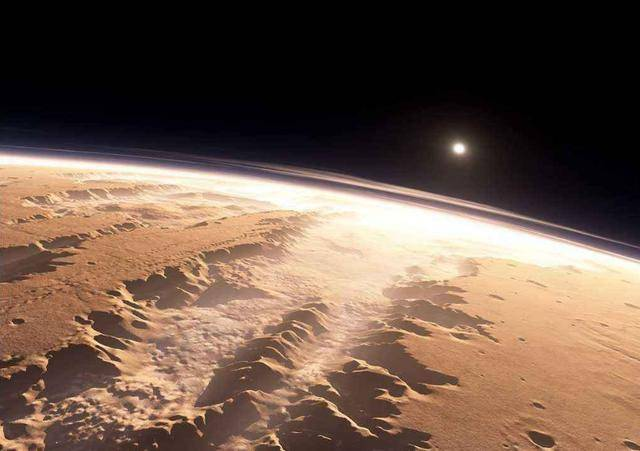
\includegraphics[width=0.6\linewidth]{火星大气环境.png}
		\caption{火星环境示意图}
		\label{fig}	
	\end{figure}
	\subsubsection{火星重力场模型}
	
	火星的质量为$6.578\times10^{23}\mathrm{kg}$,是地球质量的大约$10\%$。[3]火星的质量分布不均匀,由此导致重力场的异常。对于轨道飞行器而言,这种异常会造成扰动。
	
	行星重力场的描述模型通常用球谐函数表示,\textit{Journal  of Geophysics Research}上曾经发表过阶数为$12\times12$的火星重力场模型。
	
	为了减少计算量,在最初的分析中,本作品先假定火星质量分布较为均匀,故使用万有引力定律求解火星重力场。
	
	由万有引力定律
	
	\begin{equation}
		F=\frac{GMm}{r^2}
	\end{equation}
	
	得到引力关于飞行器与火星距离的函数
	
	\begin{equation}
	F(h)=\frac{6.67\times10^{-11}\mathrm{N\cdot m^2/kg^2}\times6.578\times10^{23}\mathrm{kg}\times m}{(h+R)^2}
	\end{equation}
	
	通过这个函数,就能够对飞行着陆器EDL过程中各高度所受引力大小进行表示。
	
	\subsubsection{火星大气密度模型}
	
	火星大气密度是火星EDL过程的重要环境参数,是火星着陆系统设计与着陆过程仿真的主要大气参数,尤其在进入段,大气密度会直接影响气动力。
	
	火星大气模型包括两类:火星大气数据库和火星大气简化模型。火星大气数据库根据火星大气环流模型和深空探测任务数据构建而成,精确性较高,但计算成本较大。火星大气简化模型是基于火星大气数据库的数据拟合后得到的指数模型,使用简单,计算难度小,适合实时仿真。[5]
	
	由于后续要求解的优化问题动态性强,故本作品使用火星大气简化模型进行计算。
	
	日本大学的Ushijima在2010年基于Mars-GRAM拟合的模型较好,其表达式为		

	\begin{equation}
		T=\left\{\begin{aligned}
			&241.0-0.999(h/1000),h<7000\mathrm{m}\\
			&249.5-2.22(h/1000),h\geq7000\mathrm{m}
		\end{aligned}\right.
		\end{equation}
		
		\begin{equation}
			P=700e^{-0.09(h/1000)},\rho=P/188.95110711075T
		\end{equation}
		
		这一模型对于两万米以下的大气情况拟合较好,但对于本作品问题的研究范围是不够的。通过MCD数据库可以获取天问一号着陆当天的大气数据。
		
\begin{figure}[htb]
			\centering
			\includegraphics[width=0.7\linewidth]{density.png}
			\caption{大气密度数据}
			\label{fig}	
\end{figure}
利用Python进行多项式拟合,就能得到大气密度的拟合。
\begin{figure}[htb]
	\centering
	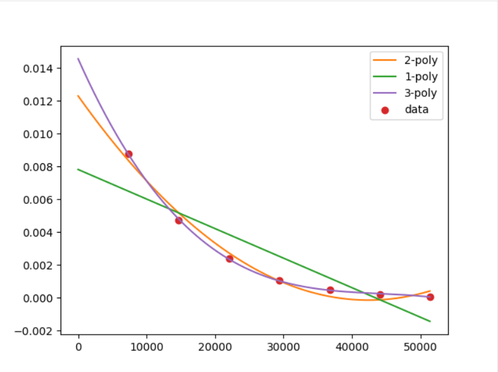
\includegraphics[width=0.6\linewidth]{大气密度拟合.png}
	\caption{大气密度多项式拟合}
	\label{fig}	
\end{figure}

其中,三次拟合效果较优。其拟合式为

\begin{equation}
\rho=-1.58370399\times10^{-16}h^3+ 2.08948544\times10^{-11}h^2 -9.38428798\times10^{-7}h+1.45762615\times10^{-2}
\end{equation}
\newpage

考虑到火星简化大气模型一般都使用指数模型进行模型,为了形式上的统一,本作品还使用Excel获得了指数拟合曲线。
\begin{figure}[htb]
	\centering
	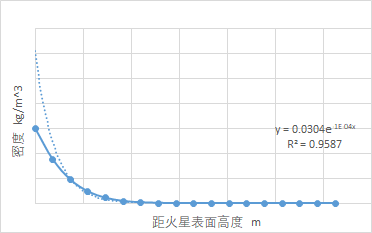
\includegraphics[width=0.6\linewidth]{exc密度拟合.png}
	\caption{大气密度指数拟合}
	\label{fig}	
\end{figure}
\begin{equation}
	\rho=0.0304e^{-10^{-4}y},20000\mathrm{m}\leq h<125\mathrm{km}
	\end{equation}
	
	拟合结果$R^2$为$0.9587$,适合仿真。
	
	综上所述,火星大气密度场模型可以描述为
	
	\begin{equation}
	\rho=\left\{\begin{aligned}
		&700e^{-0.09(h/1000)}/\{188.95[241.0-0.999(h/1000)]\},h<7000\mathrm{m}\\
		&700e^{-0.09(h/1000)}/\{188.95[249.5-2.22(h/1000)]\},7000\mathrm{m}\leq h<20000\mathrm{m}\\
		&0.0304e^{-10^{-4}h},20000\mathrm{m}\leq h<125\mathrm{km}
	\end{aligned}\right.
	\end{equation}
	\subsection{飞行器着陆轨迹建模}

建立飞行器着陆火星的轨迹模型需要考虑飞行器的位置、运动状态、受力情况。本作品使用的大量数据来源于天问一号工程叶培建院士的公开讲座内容。
\begin{figure}[htb]
	\centering
	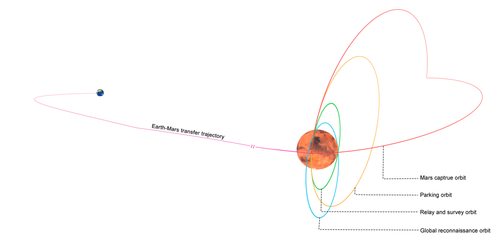
\includegraphics[width=0.9\linewidth]{飞行器着陆轨迹.png}
	\caption{飞行器飞行轨道示意图}
	\label{fig}	
\end{figure}

由于飞行着陆器EDL过程是在火星的附近,相距地球、太阳和其他星球甚远,所以可以在求解中忽略除火星外其他天体对着陆器的作用。

天文观测中使用的火心固定坐标系是非惯性的,包含了公转、自转。在EDL过程中,由于全过程时间不超过十分钟,所以可以不考虑公转及自转。 

进一步地,假定着陆轨道是从近火点出发。为了便于求解,先考虑简化坐标。本作品假定飞行着陆器进入大气位置、着陆位置、火星形心三点均在EDL过程的轨迹平面上。即利用上述三点就可以刻画出EDL过程平面。

\begin{figure}[htb]
	\centering
	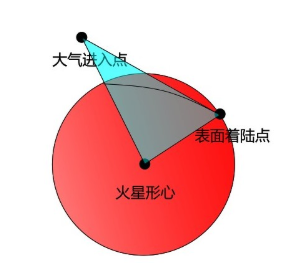
\includegraphics[width=0.4\linewidth]{EDL.png}
	\caption{共面假设示意图}
	\label{fig:pathdemo}	
\end{figure}
以飞行器指向火星形心方向作为竖直方向,就可以将运动做正交分解。EDL过程中各个阶段的切换主要由竖直方向的位置控制,这样的处理极大地方便了建模和求解。

\begin{figure}[htb]
	\centering
	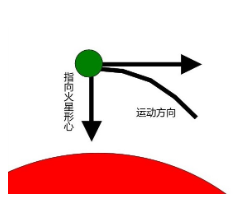
\includegraphics[width=0.5\linewidth]{坐标示意.png}
	\caption{坐标示意图}
	\label{fig:pathdemo}	
\end{figure}

\subsubsection{大气进入段轨迹动力学建模}

在这一阶段,飞行器受到火星的引力和火星大气对飞行器的阻力。其中,引力方向竖直向下,即简化坐标中的指向火星形心的竖直方向;大气阻力方向与当前运动方向相反。

\begin{figure}[htb]
	\centering
	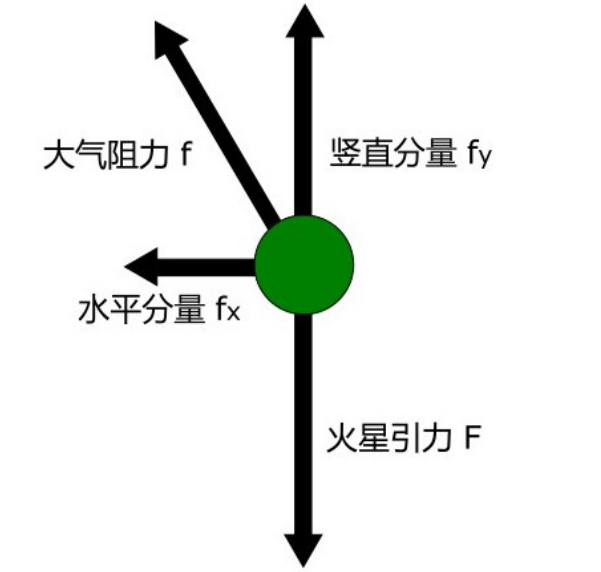
\includegraphics[width=0.5\linewidth]{受力分析.png}
	\caption{进入段受力分析示意图}
	\label{fig:pathdemo}	
\end{figure}

在相关研究中,大气阻力可用飞行器表面积、速度大小、大气密度以及阻力系数描述。

\begin{equation}
f=\frac12\rho v^2S\cdot C_D
\end{equation}

于是可知,大气进入段飞行着陆器的运动状态有以下条件

\begin{equation}
\begin{aligned}
	&f=\frac12\rho(v_x^2+v_y^2)S\cdot C_D\\
	&\beta=\arctan\frac{v_x}{v_y}\\
	&f_x=\sin\beta\cdot f\\
	&f_y=\cos\beta\cdot f\\
	&F=\frac{GMm}{(h+R)^2}
\end{aligned}
\end{equation}

其中,$\rho$为大气密度,$S$为飞行器表面积,$C_D$为阻力系数,$\beta$为运动方向角。进一步地可以得到竖直与水平两个方向上的加速度大小

\begin{equation}
\begin{aligned}
	&a_x=\frac{f_x}{m_{飞行器}}\\
	&a_y=\frac{f_y-mg}{m_{飞行器}}
\end{aligned}
\end{equation}

根据飞行器的运行轨道可以得到进入大气时的初始状态

\begin{equation}
\begin{aligned}
	&v_{x_0}=4694.61\mathrm{{m}/{s}},v_{y_0}=956\mathrm{{m}/{s}}\\
	&x_0=0\mathrm{m},y_0=125\mathrm{km}\\
	&a_{x_0}=a_{y_0}=0\mathrm{m/s^2}
\end{aligned}
\end{equation}

\begin{figure}[htb]
	\centering
	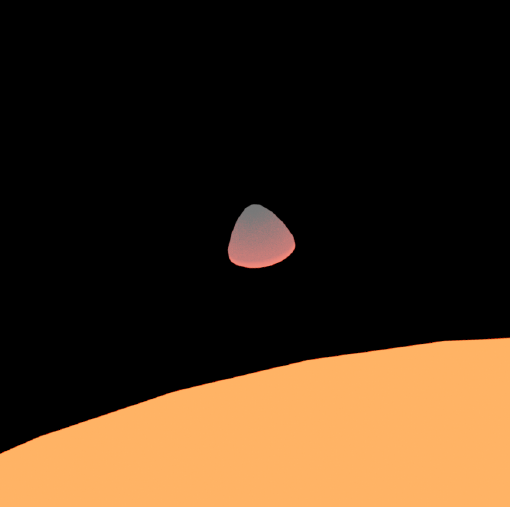
\includegraphics[width=0.5\linewidth]{大气进入过程.png}
	\caption{大气进入段示意图}
	\label{fig:pathdemo}	
\end{figure}
从进入火星开始到降落伞开伞完成,探测器
的速度从每秒几千米迅速减小到每秒几百米,这
个过程主要是靠探测器的气动外形减速的。而由
于火星大气稀薄,与在地球着陆相比,相同的有
效载荷质量需要更大的直径外形结构,体积和质
量也会相应的增加 ;此外,火星大气成分主要为
二氧化碳。在进入过程中,探测器穿过火星大气,
会产生大量的摩擦热,这就对探测器外部的防热
材料提出了更高的要求。

进入火星的气动减速和热防护外形都是由探
测器的弹道系数$\beta$决定的,研究得到, $\beta$越小,
则经气动减速后探测器所能达到的稳降速度越
小。而我们有飞行器的阻力系数:
\begin{equation}
	C_D=\frac{M}{\beta A}
\end{equation}
式中,M为探测器质量,$C_D$表示阻力系数,
A为有效面积。
为充分发挥探测器的气动减速作用,使稳降
速度尽可能减小,即令$\beta $减小,在探测器质量
一定的情况下,就要使阻力系数和有效面积增大。
因而,一般采用半锥角较大(头部较钝)的球锥
形,一方面阻力系数随着半锥角的增大而增大,另一方面头部钝度越大则气动摩擦热越小。


目前的几种火星飞行探测器的气动外形参数如下图:
\begin{figure}[htb]
	\centering
	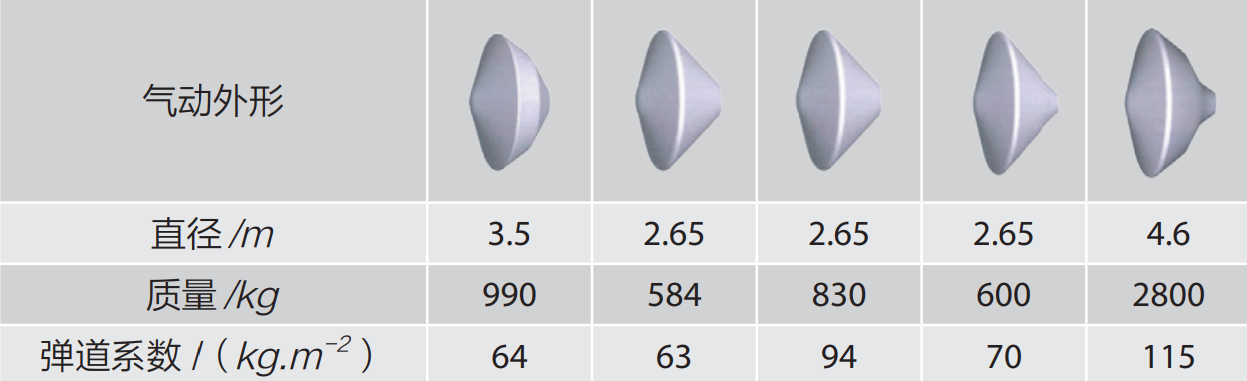
\includegraphics[width=0.8\linewidth]{气动外形.png}
	\caption{气动外形参数图}
	\label{fig:pathdemo}	
\end{figure}


依据天问一号总工程师叶培建院士所做的公开讲座,可以得到天问一号着陆飞行器的一些基本数据。

\begin{equation}
m_{飞行器}=1285\mathrm{kg},
S=12.56\mathrm{m^2},
\end{equation}
从而根据此数据大致可以得到着陆飞行器的气动外形形状以及阻力系数大小。

这样,天问一号在整个大气进入段的运动状态都是可知的。

\subsubsection{伞降减速段轨迹动力学建模}

伞降减速阶段的受力情况与大气进入段大体相似。
\begin{figure}[htb]
	\begin{minipage}[t]{0.5\textwidth}
		\centering
		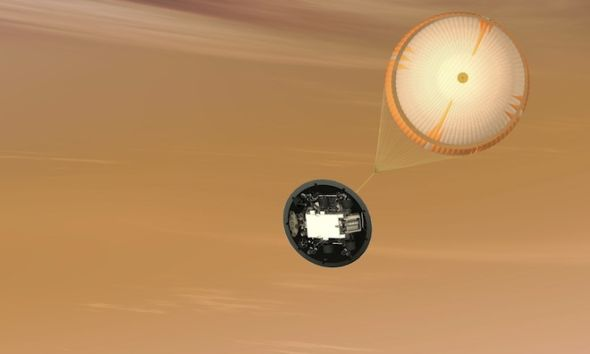
\includegraphics[scale=0.4]{伞降控制.png}
		\caption{伞降控制示意图\label{fig:1}}
	\end{minipage}
	\qquad
	\begin{minipage}[t]{0.5\textwidth}
		\centering
		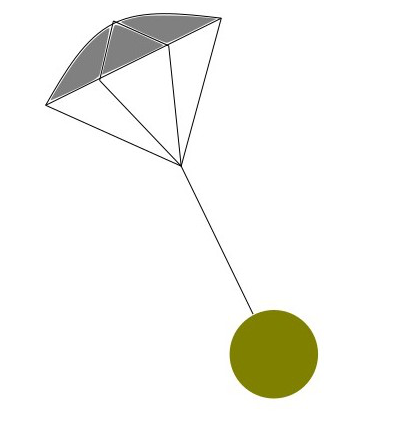
\includegraphics[scale=0.5]{降落伞减速.png}
		\caption{伞降减速模型\label{fig:2}}
	\end{minipage}
\end{figure}

大气阻力都可以用式(8)来确定。不同之处在于,此时还需要考虑降落伞提供的阻力。降落伞的表面积经估算为$200\mathrm{m^2}$。阻力系数参考既往火星探测任务:
如下表1:

\begin{table}[htb]
	\caption{降落伞阻力系数}
	\centering
		\begin{tabular}{cccc}
		\toprule
		降落伞类型& “海盗号”降落伞& “火星探路者”降落伞	& “火星探测漫游者”降落伞\\
		\midrule
		阻力系数& 0.67&0.41&0.43\\
		\bottomrule %添加表格底部粗线
		\end{tabular}
		\end{table}

		从而本作品中降落伞阻力系数取$0.43$。

而开伞条件为

\begin{equation}
Mach=2,
h>4\mathrm{km}
\end{equation}

\subsubsection{发动机制动段动力学建模}
在 EDL 过程中,动力下降过程是最后一个阶段,通过主发动机和姿控发动机
的控制,使着陆器安全软着陆。这一阶段主要依靠发动机推力进行减速。
当着陆器海拔在$1.5\mathrm{km}$时,就进入到发动机制动阶段。

记发动机在水平方向和竖直方向的推力分量分别为$u_x(t)$和$u_y(t)$。着陆器在$t$时刻质量为$m(t)$。可以构建如下运动学方程。

\begin{equation}
\begin{aligned}
&m(t)\frac{\mathrm{d}^2x}{\mathrm{d}t^2}=u_x(t)\\
&m(t)\frac{\mathrm{d}^2y}{\mathrm{d}t^2}=\frac{GMm(t)}{(R+y(t))^2}+u_y(t)\\
\end{aligned}	
\end{equation}

\begin{figure}[htb]
	\centering
	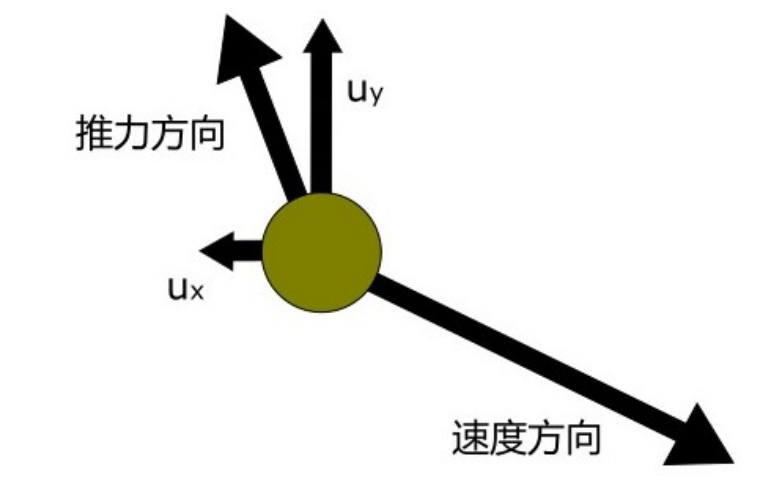
\includegraphics[width=0.6\linewidth]{发动机制动.png}
	\caption{发动机制动段示意图}
	\label{fig:pathdemo}	
\end{figure}

另外,由发动机比冲的定义可以知道

\begin{equation}
\frac{\mathrm{d}m}{\mathrm{d}t}=\frac{\sqrt{u_x(t)^2+u_y(t)^2}}{v(t)}
\end{equation}

式中右端分子部分值为$7500$N。

\subsubsection{EDL过程仿真验证}

求解优化问题之前,有必要对已建立的EDL过程模型进行编程验证。

\begin{figure}[htb]
	\centering
	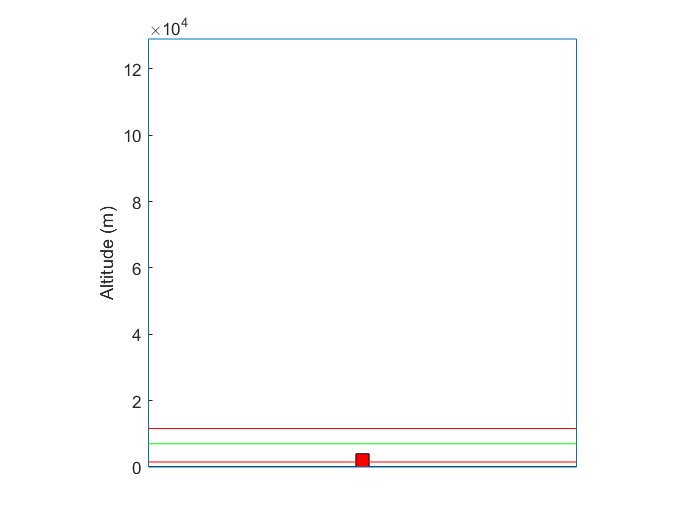
\includegraphics[width=0.6\linewidth]{仿真动画.png}
	\caption{仿真动画示意图}
	\label{fig:pathdemo}	
\end{figure}

仿真使用Matlab完成,将火星飞行器降落过程竖直方向以二维动画方式形成。仿真过程中使用竖直方向位移作为位置参数,并将水平方向位移作为结果输出。

\begin{figure}[htb]
	\centering
	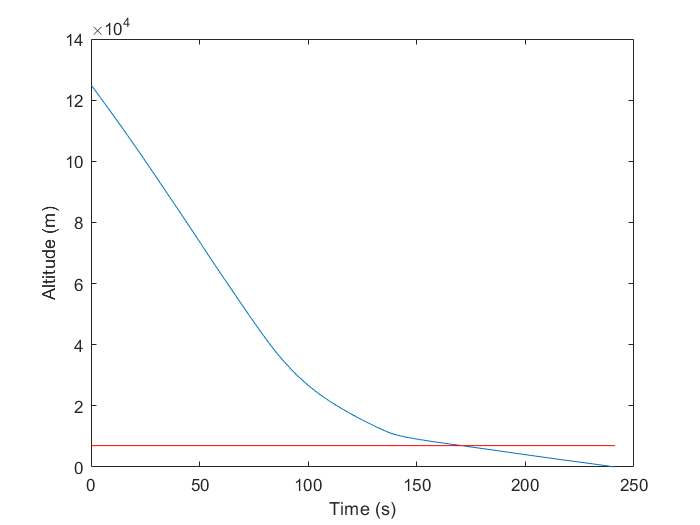
\includegraphics[width=0.6\linewidth]{海拔变化.png}
	\caption{海拔变化}
	\label{fig:pathdemo}	
\end{figure}

\section{轨迹设计}



\subsection{初始点位置估计}
如图16所示的火星表面无旋转的固连坐标系作为参考坐标系。该坐
标系的原点位于目标着陆点,三轴方向分别为横向、侧向及高度方向。

\begin{figure}[htb]
	\centering
	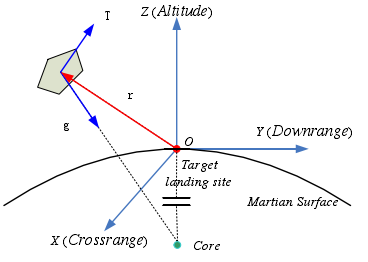
\includegraphics[width=0.6\linewidth]{参考坐标系.png}
	\caption{参考坐标系示意图}
	\label{fig:pathdemo}	
\end{figure}

由于天问一号着陆器与环绕器分离点位置坐标并未公布。还不能够求解优化问题。根据前期仿真验证结果,可以得到着陆器在水平方向上的位移。

\begin{figure}[htb]
	\centering
	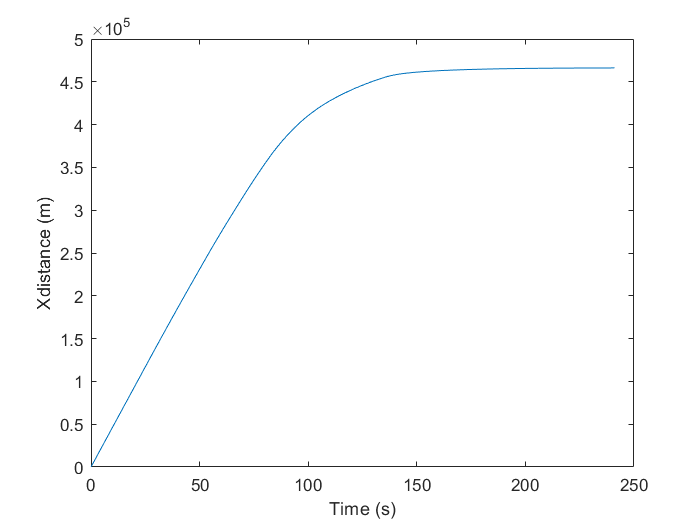
\includegraphics[width=0.6\linewidth]{水平位移.png}
	\caption{水平位移}
	\label{fig:pathdemo}	
\end{figure}

火星飞行器的着陆准备轨道与火星赤道平面倾角为$86.9^{\circ}$,环绕方向与火星自转方向一致。所以知道分离点在着陆点西南方,且可以推知分离点经度近似于着陆点。

在探测任务前期规划中,轨道平面倾角被设定为$90\pm5^\circ$。不妨假定轨道平面垂直于赤道平面。于是着陆器在水平方向位移就反映了着陆器EDL过程中的纬度变化。

由火星半径可以知道,火星上纬度差为$1^\circ$的两点距离为

\begin{equation}
	\frac{\pi R}{180}=59166.66\mathrm{m}
\end{equation}

根据累积位移可以求得纬度差为$28.7^\circ$。于是分离点经纬度坐标为($3.6^\circ S$,$109.9^\circ E$)。

\subsection{着陆点估计}
火星表面遍布斜坡、高山、岩石、巨大的火
山坑、沟壑等障碍物,地形非常复杂。因而在着陆
时,需要精确合理的选择着陆位置,这就要求探测
器具有实时对着陆地区障碍地形和着陆点进行检
测、评估及轨迹规划、制导的能力。此外,由于
火星表面温度分布不均,大气运动十分剧烈,因
而常常有尘暴现象出现,其平均风速可达 50m/s。
这就对减速装置及着陆稳定性的设计有较高要求。

对于火星飞行器着陆点的估计,本作品认为需要从这几方面考虑:

第一,着陆区的地形要平坦,这就决定了着陆点很可能位于火星的北半球,在火星北半球有着较大面积的平原,北半球的整体海拔高度相对南半球都要低一些;

第二,着陆区需要有科学考察的意义,从而火星上有水、海洋的地方需要被优先考虑,美国宇航局发射了4代火星车,全部都冲着火星上可能有生命的地方,比如好奇号降落在盖尔撞击坑,坑中有一座5000多米海拔的夏普山,这座山被认为曾经被海洋覆盖到半山腰的位置,有可能存在生命;
勇气号和机遇号降落在古塞夫撞击坑和子午线平原,子午线平原上有灰色的结晶赤铁矿,在地球上,这种矿物形成于温泉或者静水湖泊中,子午线平原上的赤铁矿厚度可达到数百米之巨。古塞夫撞击坑被认为是古老的湖床,还有火山喷发的痕迹,这说明这里是一处火山湖,研究价值较高。

结合火星地图(如图18)以及天问一号的着陆报道,
最终我们选定飞行器在乌托邦平原着陆,经纬度坐标为($25.1^\circ N$,$109.9^\circ E$)。

NASA中火星上功能强大的HiRISE摄像机的首席研究员Alfred McEwen表示:该地点“大多平坦而光滑,但有火山口,风成的风脊和一些巨石。”该地区被一些科学家解释为被泥石流覆盖,因此可能存在古老的深层地下水,这可能是一个与流浪者一起研究的有趣地点。乌托邦平原高度低,这意味着进入太空飞船将有更多的时间和气氛减速并安全地下降到地面,而且这里是太阳系中最大的撞击盆地,也具备探索价值。[8]
\begin{figure}[htb]
	\centering
	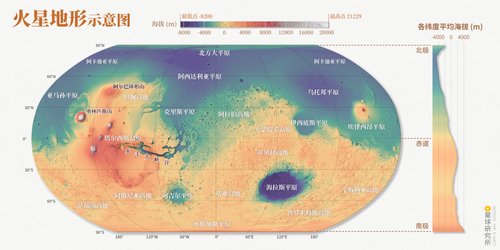
\includegraphics[width=0.8\linewidth]{火星地形图.png}
	\caption{火星地形示意图}
	\label{fig:pathdemo}	
\end{figure}

\newpage
\subsection{时间最优控制方案设计}
\subsubsection{遗传算法求解轨迹}

注意到,EDL过程中可以通过预设方案进行控制的部分只有发动机制动段。所以只需求解发动机制动段的最优方案。

不妨假定发动机始终以最大推力运作,在制动过程中着陆器仅受到发动机推力和火星引力。于是有

\begin{equation}
	\left\{
\begin{aligned}
	&m(t)\frac{\mathrm{d}^2x}{\mathrm{d}t^2}=u_x(t)\\
	&m(t)\frac{\mathrm{d}^2y}{\mathrm{d}t^2}=\frac{GMm(t)}{(R+y(t))^2}+u_y(t)\\
	&\frac{\mathrm{d}m}{\mathrm{d}t}=\frac{7500}{v_e}
\end{aligned}\right.
\end{equation}

而约束条件有

\begin{equation}
\left\{\begin{aligned}
&\sqrt{u_x^2+u_y^2}=7500\\
&m(0)=1285\\
&x(0)=0,y(0)=1192.56\\
&\frac{\mathrm{d}x}{t}|_{t=0}=2.2\\
&\frac{\mathrm{d}y}{t}|_{t=0}=95.1\\
&y(t_f)=-100\\
&\sqrt{{\frac{\mathrm{d}x}{t}|_{t=t_f}}^2+{\frac{\mathrm{d}x}{t}|_{t=t_f}}^2}=3.6
\end{aligned}\right.
\end{equation}

在本策略中,目标泛函为$J=t_f$。显然,这是一个Mayer型泛函。[12]状态变量为着陆器的位置参数、运动状态等,控制变量是水平和竖直两个方向上的推力分量。

如果记着陆器方向角为$\theta$,那么可以得到控制变量的更精确形式

\begin{equation}
	\left\{
	\begin{aligned}
		&u=a_1t^3+a_2t^2+a_3t+a_4\\
		&\theta=b_1t^3+b_2t^2+b_3t+b_4
	\end{aligned}
	\right.
\end{equation}

可以将$u_x$及$u_y$表成$u\cos\theta$及$u\sin\theta$。根据该阶段所处的状态,大体估计出该阶段所需要的时间小于90秒。因此,将时间段在[0,90]内进行离散化,采用四阶Runge-Kutta方法进行参数范围的估计,见表2。

\begin{table}[h]
	\centering
	\begin{tabular}{ccc}  
		\toprule   
		\heiti 参数&\heiti 下界&\heiti 上界\\  
		\midrule   
		$a_1$&-10&10\\
		$a_2$&-10&10\\
		$a_3$&-100&100\\
		$a_4$&1500&10000\\
		$b_1$&-10&10\\
		$b_2$&-10&10\\
		$b_3$&-10&10\\
		$b_4$&-100&100\\
		\bottomrule  
	\end{tabular}
\caption{参数估计}
\end{table}

在此基础上,利用遗传算法求解时间最优的控制方案。优化变量个数为8,每代种群数量为50,迭代1000次,变异概率为0.01。解得最优时间为14.28秒,参数结果见表3。

\begin{table}[h]
	\centering
	\begin{tabular}{c}  
		\toprule   
		\heiti 变量\\  
		\midrule   
		$u=-7.1t^3+90.3t^2+89.4t+5134$\\
		$\theta=9.4t^3-3.6t^2+2.9t-24.4$\\
		\bottomrule  
	\end{tabular}
\caption{优化变量}
\end{table}


\subsection{燃料最优控制策略求解}

动力下降阶段,发动机主要任务是抵消着陆器的初始动能和势能。在实际制动中,为了实现精准降落的目的,发动机的推力方向会随时间变化,不同时刻的推力大小也不同,但仍处于发动机推力的变化范围中。[13]除此之外,随着燃料的消耗,着陆器本身的质量也会随之降低。

由以上特点,我们建立如下的优化模型:

\begin{equation}
	\begin{aligned}
	\min\quad&J(u,\theta)=\int^{t_f}_0\frac{u}{v_e}\mathrm{d}t\\
	\mathrm{subject\enspace t}o\quad&(18-19)
	\end{aligned}
\end{equation}

\subsubsection{策略求解}

显然,目标泛函是一个Bolza型泛函[12]。由于控制变量$\theta(t)$和$u(t)$的搜索空间是一个泛函空间,无法直接应用优化算法,因此首先我们将这个轨迹优化问题转化为参数优化问题。即用多项式来表示控制变量,如(20)。

这样轨迹优化问题就转化为对多项式系数的优化。但是,这些参数并没有明确的物理意义,确定初值及搜索空间比较困难。因此我们采用离散化的方法对优化问题进行改进。

首先将火星着陆器动力下降轨迹离散化分割成 n 个小段,每段的节点设定一个推力大小和方向角,那么可以将n+1个节点的推力大小和方向角作为待优化的参数。每个节点的时刻可以由下式得到:

\begin{equation}
	t_i=t_0+i(t_f-t_0)/n
\end{equation}

这样,就使得每个节点的推力大小和方向角都有一个对应的节点时刻。那么利用这n+1个节点的推力大小和方向角及对应时刻,对式(20)进行拟合,可以求得多项式的 各项系数,进而得到整个动力下降轨迹的推力大小和方向角的曲线。

\subsubsection{十进制蚁群优化算法求解}

对燃料的优化问题本质上是一个二元函数连续优化的问题,上述数学模型可以简化为:

\begin{equation}
	\begin{aligned}
		\min\quad&J(u,\theta)\\
		\mathrm{subject\enspace to\quad}&u\in[u_0,u_1],\theta\in[\theta_0,\theta_1]
	\end{aligned}
\end{equation}

先通过变换将优化参数的变化范围转化为[0,1]。设转换后的优化参数x要求精确到小数点后d位,则该优化参数值可以用1+d个十进制数字来构成

这里构造1+d×10个城市如图19所示其结构为1+d列第一列代表个位上的数这一列只有一个城市代表个位上只能选的数字0。其余 d 列从左至右分别代表小数点后十分位、百分位、千分位等每列包括10个城市分别代表每个数位上可选的0到9这10个十进制数字。

\begin{figure}[htb]
	\centering
	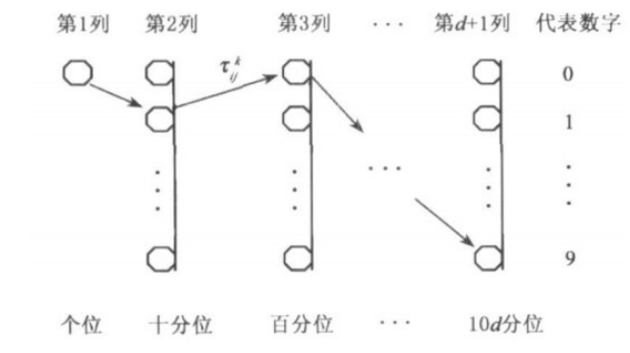
\includegraphics[width=0.7\linewidth]{城市群构造.png}
	\caption{城市群构造}
	\label{fig:pathdemo}	
\end{figure}


蚂蚁在这样的城市群上选择路径时根据一定的路径转移规则从左向右走每列上必须且只能选择一个城市。这样蚂蚁从左到右完成一个循环以后走过的路径包含有1+d个城市它们所代表的数字可以构成一个在[0,1]上有 d 位有效数字的小数。经过路径解码后,成为优化参数的一个可行解。

所有蚂蚁完成一次循环后要根据信息素更新规则更新相关路径上的信息素量。使蚂蚁经过多次循环之后,逐渐向最优路径聚集,也就是优化参数逐渐向最优解收敛。

用参数化方法的相关参数设置为:设将轨迹离散化为9段,那么待优化参数共20个参数即10个推力方向角和10个推力大小。在用蚁群算法进行优化过程中需要确定这20个优化参数的搜索范围。对于10个方向角,由经验可知,推力方向与水平方向夹角不会超过180度,否则着陆器将会被加速,燃料消耗将更多。

综上,本算例中算法参数应设置为:

\begin{table}[ht]
	\centering
	\begin{tabular}{cccccc}  
		\toprule   
		\heiti num-ant&\heiti num-clc&\heiti K&\heiti Q&\heiti $\rho$&$\tau_0$\\  
		\midrule   
		1000&50&5&0.5&0.2&5\\
		\bottomrule  
	\end{tabular}
	\caption{蚁群参数}
\end{table}

按照前述方法用十进制蚁群算法对火星软着陆轨迹进行优化。由于十进制蚁群算法是基于概率转移的仿生算法,优化结果具有一定的随机性,所以这里进行了10次仿真,结果全部收敛,证明在本方案中,十进制蚁群算法具有良好的收敛性。

由十进制蚁群算法得到的优化参数见表5,由于参数过多,故不一一列出。

\begin{table}[ht]
	\centering
	\begin{tabular}{cccccccc}  
		\toprule   
		\heiti $u_1$&\heiti $u_2$&\heiti $\cdots$&\heiti $u_{10}$&\heiti $\theta_1$&\heiti $\theta_2$&\heiti $\cdots$&\heiti $\theta_{10}$\\  
		\midrule   
		3280&4493&$\cdots$&2105&32.86&45.72&$\cdots$&88.08\\
		\bottomrule  
	\end{tabular}
	\caption{蚁群参数}
\end{table}

将以上20个优化参数投入到参数化方法中的多项式中,我们可以得到发动机推力大小和方向角随时间变化曲线和参数。见图20及表6。

\begin{figure}[htb]
	\centering
	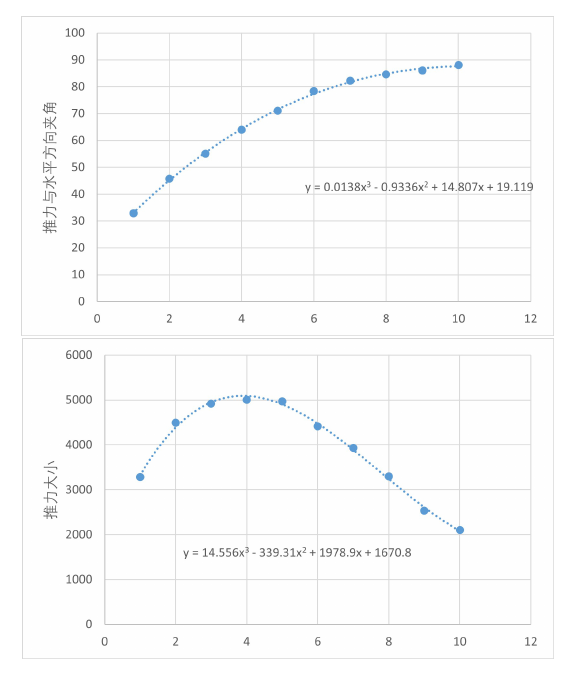
\includegraphics[width=0.6\linewidth]{推力.png}
	\caption{推力方向角及大小变化}
	\label{fig:pathdemo}	
\end{figure}


\begin{table}[ht]
	\centering
	\begin{tabular}{c}  
		\toprule   
		\heiti 变量\\  
		\midrule   
		$u=14.556t^3-339.31t^2+197.9t+5134$\\
		$\theta=0.0138t^3-0.9336t^2+14.807t+1670.8$\\
		\bottomrule  
	\end{tabular}
	\caption{优化变量}
\end{table}

将上述结果代入动力学模型中,我们最终可以得到,动力下降阶段燃料消耗为$\Delta m=168.33\mathrm{kg}$。



\subsection{误差控制分析}

飞行器在实际着陆的控制过程中,往往客观存在一定的控制误差,譬如着陆准备轨道参数(近月点位置和速度)的误差、发动机推力(大小和方向)的控制误差、模型的简化假设和近似求解误差等。 诸如这些误差势必会对实际的轨道设计和控制结果造成或多或少的影响,从工程应用的角度需要做相应的敏感性分析。而且涉及到的相关参数,如坐标系的选取、变量的选择、参数的选取、约束条件、函数 的简化和月面的观测等都存在一定的偏差,那么对轨道设计和控制策略的影响程度如何,也需要就某些情况做相应的敏感度分析。

这里仅就主减速发动机推力变化的敏感性进行分析。

主发动机最大推力的误差影响 对于主减速阶段,主发动机要求以7500N最大推力运行,但事实上发动机的推力和实际推力会有一些误差。
           
主发动机推力方向角近似控制多项式系数误差的影响主发动机推力方向角的控制函数是用三次多项式来实现的,其系数是根据各阶段的状态要求通过数值方法搜索得到的,势必也存在一定的误差。
 
飞行器的运行状态对方向角的控制多项式系数的改变是非常敏感的,尤其是 对运行轨迹和高度的影响较大,但对速度无影响。因此,在实际中需要提高该参数的传输和控制的精度,才能保证实际需求。 

对于其他参数的敏感性分析,方法是类似的,这里不再赘述。

\section{作品设计的创新点}
本作品提出的解决方案对飞行器轨迹设计是较为适恰的。经过前期大量地对数据进行收集和处理,我们得到了解决本问题所必需的各项数据。在动力学建模阶段,我们通过对问题适当的简化并基于物理学分析,较为准确地建立了飞行着陆器EDL过程动力学模型。

求解时间最优控制策略方案时,由于已知的路径点过少,本作品选择了智能优化算法求解。这类算法不能保证所得结果是全局最优的。事实也是如此,天问一号EDL过程中与地球无通信,其状态无从获知。该问题的解即便最优,也未必就符合实际情况。回到方法的讨论上,在本问题中遗传算法的收敛性较好,在1000次迭代中就得到了结果。

在考虑燃料最优控制策略方案的求解时,本作品采用了对整个动力下降过程进行一定程度上的离散化,再利用十进制蚁群算法对20个优化参数基于概率转移进行求解,在进行多次仿真后,结果全部收敛,说明在本方案中,十进制蚁群算法具有良好的收敛性。由此,我们可以考虑将十进制蚁群算法推广到其他优化模型中,解决了蚁群算法很难对连续目标函数进行优化的问题,且该方法具有良好的收敛性,值得在其他问题中尝试、应用。

在本次求解过程中,我们发现燃料最优模型结果对轨迹离散化处理程度有一定的要求,仅将动力下降过程离散为10个过程,很难使模型具有较高的精度,因此会出现一定的误差。但如果要提高精度就会带来难以预测的计算量。这表明本作品的算法仍然有改进的空间。
\newpage
\section{论文/报告的引用和发表}
	\begin{flushleft}
		\fontsize{10.0pt}{0}
		[1]\enspace 新华社.五大看点!这份中国首次自主火星探测任务“观赏指南”请收好.[EB/OL].\url{http://www.xinhuanet.com/2020-07/23/c_1126275770.htm}, 2021-08-07
		
		[2]\enspace 新华社.习近平代表党中央、国务院和中央军委祝贺我国首次火星探测任务天问一号探测器成功着陆火星的贺电.[EB/OL].\url{http://www.xinhuanet.com/2021-05/15/c\_1127448736.htm}, 2021-08-07
		
		[3]\enspace 欧阳自远,肖福根.火星及其环境[J].航天器环境工程,2012,29(06):591-601.
		
		[4]\enspace Christensen E J, Balmino G. Development and analysis of a twelfth degree and order gravity model for Mars[J]. Journal of Geophysics Research, 1979, 84: 7943-7945
		
		[5]\enspace 秦同,王硕,高艾,朱圣英,崔平远.一种火星大气密度三维解析模型[J].深空探测学报,2014,1(02):117-122.
		
		[6]\enspace Ushijima M,  Hara H,  Muramatsu A,et al. The operating characteristics of a ducted rocket in the Mars atmosphere [J].AIAA paper, 20106999.
		
		[7]\enspace 欧洲航天局.MCD数据库.[DB].\url{http://www-mars.lmd.jussieu.fr/mcd_python/}, 2021-08-07
		
		[8]\enspace 航天爱好者网.2020中国火星探测计划(根据叶院士报告整理).[EB/OL]. \url{http://www.spaceflightfans.cn/28219.html}, 2021-08-07
		
		[9]\enspace 陈旭,荣伟,陈国良. 大气对降落伞开伞动载阻尼作用的分析[A]. 中国科学技术协会.提高全民科学素质、建设创新型国家——2006中国科协年会论文集(下册)[C].中国科学技术协会:中国科学技术协会学会学术部,2006:5.
		
		[10]于莹潇,田佳林.火星探测器降落伞系统综述[J].航天返回与遥感,2007(04):12-16.
		
		[11]人民日报.祝融号火星车顺利发回遥测信号 我国首次火星探测任务着陆火星成功.[EB/OL].\url{http://finance.people.com.cn/n1/2021/0515/c1004-32104220.html}, 2021-08-07
		
		[12]雍炯敏.最优控制教程[M].第1版.北京:高等教育出版社,2006.
		
		[13]杜剑平,韩中庚.嫦娥三号软着陆轨道设计与控制策略的优化模型[J].数学建模及其应用,2014,3(04):39-53.
		
		[14]戴娟. 火星着陆器轨迹跟踪控制方法研究[D].北京理工大学,2016.

		[15]张瑶. 火星探测器动力下降段软着陆制导研究[D].哈尔滨工业大学,2018.
	
		[16]崔平远,胡海静,朱圣英.火星精确着陆制导问题分析与展望[J].宇航学报,2014,35(03):245-253.
	
		[17]任高峰,朱圣英.火星着陆任务落点误差快速分析方法[J].哈尔滨工业大学学报,
		
		2012,44(07):14-20.
		[18]王超,徐瑞. 基于时间-燃耗优化的火星反推制动制导律设计[A].中国宇航学会深空探测技术专业委员会,2013:6.
		
		[19] Wolf A A, Graves C, Powell R, et al. Systems for pinpoint landing at Mars[J]. 2004.
	
	\end{flushleft}
	\newpage
	\section{附件(视频或3D模型等)}
\subsection{程序附录}
	\lstinputlisting[
		style       =   python,
		caption     =   {\bf guidaomini.py},
		label       =   {guidaomini.py}
	]{C:/Users/15526/Desktop/先进飞行器虚拟仿真/guidaomini.py}

	\lstinputlisting[
		style       =   python,
		caption     =   {\bf A1sim.py},
		label       =   {A1sim.py}
	]{C:/Users/15526/Desktop/先进飞行器虚拟仿真/A1sim.py}

	\lstinputlisting[
		style       =   MATLAB,
		caption     =   {\bf DACA.m},
		label       =   {DACA.m}
	]{C:/Users/15526/Desktop/先进飞行器虚拟仿真/DACA.m}

	\lstinputlisting[
		style       =   MATLAB,
		caption     =   {\bf odeRK4.m},
		label       =   {odeRK4.m}
	]{C:/Users/15526/Desktop/先进飞行器虚拟仿真/odeRK4.m}
	\subsection{视频等资料附录}
	见附件文件夹中.avi等格式附件。
\end{document}




